\documentclass[12pt,a4paper,openright,twoside]{book}
\usepackage[utf8]{inputenc}
\usepackage{phd-thesis}

\mainlinespacing{1.241} % line spacing in mainmatter, comment to default (1)

\begin{document}
	
\frontmatter
%!TeX root = phd-thesis.tex
\title{Symbolic Knowledge Injection \& Extraction for Autonomous Learning}
\author{Matteo Magnini}
\date{\today}

\newgeometry{margin=0.8in}
\begin{titlepage}
	\begin{center}
		% \vspace*{0.2cm}

		\large
		\textbf{ALMA MATER STUDIORUM -- UNIVERSITÀ DI BOLOGNA \\ DISI Dipartimento di Informatica: Scienza e Ingegneria}
		\\
		\noindent\hrulefill
		\vspace{0.4cm}

		\Large
		Doctor of Philosophy in \\
		Computer Science and Engineering

		\vspace{0.4cm}

		Cycle XXXVIII

		\vspace{0.4cm}
		%TODO: update as soon as Ilaria provides the offcial template
		Settore Scientifico Disciplinare: ING-INF/05

		Settore Concorsuale: 09/H1

		\Huge
		\vspace{3cm}
		\textbf{
			Symbolic Knowledge Injection \& Extraction for Autonomous Learning
		}

		{\Large{
		\vspace{3cm}

		\textit{Candidate:\\}
		\centering
		Matteo Magnini}
		\\}
		\large
		\vspace{2.5cm}
		\begin{minipage}[t]{0.64\textwidth}
			\begin{flushleft}
				\textit{PhD coordinator:}
				\\
				\textbf{Prof. Ilaria Bartolini}
			\end{flushleft}
		\end{minipage}
		\begin{minipage}[t]{0.34\textwidth}
			\begin{flushright}
				\textit{Supervisor:}
				\\
				\textbf{Prof.} \textbf{Andrea Omicini}
				\\
				\vspace{0.4cm}
				\textit{Co-supervisor:}
				\\
				\textbf{Prof.} \textbf{Enrico Denti}
			\end{flushright}

		\end{minipage}\\

		\vfill
		\noindent\hrulefill
		\vspace{0.3cm}
		\Large
		%TODO: update as soon as Ilaria provides the offcial template

		Esame finale anno 2025
	\end{center}
\end{titlepage}
\restoregeometry

\begin{abstract}
    %
    \Ac{AI} represents one of humanity's most transformative technological advancements, with roots in the mid-20th century and a rapidly growing impact on society.
    %
    Over the past decade, the field of \ac{NeSy} \ac{AI}, which seeks to integrate \emph{symbolic} and \emph{sub-symbolic} approaches, has gained increasing prominence as a promising paradigm for building intelligent systems.
    %
    By combining the structured reasoning capabilities of symbolic AI with the adaptability and scalability of sub-symbolic methods, \ac{NeSy} aims to overcome the inherent limitations of each paradigm, paving the way for more robust and interpretable AI systems.

    Within \ac{NeSy}, two foundational areas of research are \ac{SKI} and \ac{SKE}, which provide the essential tools to design hybrid systems.
    %
    \Ac{SKI} focuses on injecting structured knowledge into sub-symbolic models, enabling them to leverage prior domain expertise.
    %
    \Ac{SKE}, on the other hand, facilitates the extraction of human-understandable knowledge from these models, bridging the gap between their internal representations and user interpretability.
    %
    Together, these methods offer a pathway toward developing systems that are explainable, reliable, and effective in dynamic, real-world scenarios.

    This thesis explores the challenges and opportunities of \ac{NeSy} \ac{AI}, with a particular focus on \ac{SKI}, \ac{SKE}, and their role in the engineering of intelligent systems.
    %
    After an overview of the background and state of the art, we identify key challenges in integrating symbolic and sub-symbolic paradigms.
    %
    We then present original contributions in the form of methodologies, algorithms, and tools designed to advance the capabilities of \ac{NeSy} systems.

    The advent of \acp{LLM} has further transformed the landscape of \ac{AI}, offering unprecedented capabilities for understanding and generating natural language.
    %
    This thesis investigates how \acp{LLM} can augment \ac{SKI} and \ac{SKE}, providing new avenues for designing systems that learn and adapt autonomously.
    %
    By leveraging these models, we demonstrate how hybrid approaches can address complex challenges, such as fairness and decision-making in healthcare, while ensuring interpretability and alignment with ethical principles.

    Finally, we discuss how these advancements align with the broader vision of \ac{NeSy}, while also contributing to the specific goal of this thesis: enabling the development of systems capable of fully autonomous learning.
    %
    These systems integrate the structured reasoning of symbolic AI with the adaptability of sub-symbolic models and the transformative potential of \acp{LLM}, opening pathways toward more versatile and intelligent applications.
    %
    Such progress not only advances the field but also hints at the distant horizon of general AI, bringing us closer to a future where machines can learn, reason, and adapt autonomously.

    \sloppypar
    \textbf{Keywords} -- \emph{\acl{AI}, \acl{NeSy} \ac{AI}, \acl{SKI}, \acl{SKE}, \aclp{LLM}, Intelligent Systems, Autonomous Learning.}
\end{abstract}



\begin{dedication} % this is optional
    %
    ``The work of each individual contributes to a totality, and so becomes an undying part of the totality.
    %
    That totality of human lives -- past and present and to come -- forms a tapestry that has been in existence now for many tens of thousands of years and has been growing more elaborate and, on the whole, more beautiful in all that time.
    %
    % Even the Spacers are an offshoot of the tapestry and they, too, add to the elaborateness and beauty of the pattern.
    %
    [\dots] An individual life is one thread in the tapestry and what is one thread compared to the whole?
    %
    Daneel, keep your mind fixed firmly on the tapestry and do not let the trailing off of a single thread affect you.''

    ---Isaac Asimov, \emph{Robots and Empire}
    %
\end{dedication}

\begin{acknowledgements} % this is optional

\end{acknowledgements}

%----------------------------------------------------------------------------------------
\tableofcontents   
\listoffigures     % (optional) comment if empty
\lstlistoflistings % (optional) comment if empty
%----------------------------------------------------------------------------------------

\mainmatter

%! Author = matteomagnini
%! Date = 05/03/25

%----------------------------------------------------------------------------------------
\chapter{Introduction}
\label{ch:introduction}
\mtcaddchapter
\minitoc
%----------------------------------------------------------------------------------------

\begin{refsection}

\section{Research background and context}
\label{sec:research-background-and-context}
%
Through the course of history, humanity has experienced several socio-technological revolutions that have changed the way we live.
%
From the first industrial revolution that initiated the automation of manual labor, to the world-wide spread of computers that started the automation of processes and decision-making \sidenote{cite/talk about expert systems(?)}, we are now witnessing the \ac{AI} revolution.
%
The advent of \ac{AI} has already successfully automated cognitive tasks \sidenote{add citation to image recognition and similar}, and it is expected to go further by reaching -- and possibly surpassing -- \emph{human-level intelligence}.
%
\Ac{AI} is not a recent invention, it has been around since the 1950s.
%
The reasons why only now (in the last decade to be more precise) \ac{AI} has become ubiquitous are the presence of crucial ingredients that were missing in the past.
%
Thanks to
%
\begin{inlinelist}
    \item the enormous amount of \emph{data},
    %
    \item the improvement of \emph{memory} and \emph{computational power} -- that still follows the Moore's law --, and
    %
    \item the affordability of huge quantity of \emph{energy},
    %
\end{inlinelist}
%
\ac{AI} finally flourished again.

The first kind of \ac{AI} that was developed is \emph{symbolic}.
%
Symbolic means that there are \emph{symbols} with specific \emph{meanings} that are manipulated by algorithms.
%
Symbolic \ac{AI} follows the \emph{deductive} process of reasoning, where the system starts from a set of axioms and applies rules.
%
These kinds of \ac{AI} programs are pretty effective in well-defined domains where there are clear rules that always hold, e.g., board games,~\ac{TSP},~\acp{BWP}, etc.
%
\emph{Sub-symbolic} \ac{AI} came after, and it is based on the \emph{inductive} process of reasoning.
%
Conversely to symbolic \ac{AI}, sub-symbolic \ac{AI} does not rely on symbols that have meanings for humans, but on \emph{patterns} that are learned from data.
%
Programs that uses sub-symbolic \ac{AI} to solve a certain task are said to perform \ac{ML}, because a model needs to first learn from examples before being able to generalize to unseen data.
%
\sidenote{consider to add a sentence or two about other different kinds of algorithms based on different learning principles like RL}
%
Sub-symbolic models like \acp{NN} can reach human or super-human performance in pre-defined tasks like image recognition, natural language processing, and many others.
%
However, to be properly effective, these models usually need a huge amount of data and hardware resources.

The natural evolution in \ac{AI} research is to use both symbolic and sub-symbolic approaches together.
%
This is the idea behind \ac{NeSy} \ac{AI}, where the deductive reasoning of symbolic \ac{AI} is combined with the inductive learning of sub-symbolic models, especially \acp{NN}.
%
This branch of \ac{AI} is still relatively young; the first works that tried to combine logic rules within a \ac{NN} date back to the 90s~\cite{DBLP:conf/aaai/TowellSN90,DBLP:journals/ai/TowellS94}.


\section{Overview and contributions}
\label{sec:overview-and-contributions}
%
Lorem Ipsum

\section{Structure of the thesis}
\label{sec:structure-of-the-thesis}
%
Lorem Ipsum

\printbibliography[title=Reference,heading=bibintoc]

\end{refsection}

%----------------------------------------------------------------------------------------
%--------------------------------------- PART I -----------------------------------------
%----------------------------------------------------------------------------------------

\part{Background}\label{part:background}

%! Author = matteomagnini
%! Date = 05/03/25

%----------------------------------------------------------------------------------------
\chapter{Intelligent Systems}
\label{ch:intelligent-systems}
\mtcaddchapter
\minitoc
%----------------------------------------------------------------------------------------

\section{What is intelligence?}\label{sec:what-is-intelligence}

Intelligence is a concept that encompasses a wide range of abilities and characteristics of single \emph{individuals} or \emph{groups}.
%
From an \emph{evolutionary} perspective, intelligence characterises some animal species -- and organisms belonging to other biological kingdoms -- from simple forms of life.
%
In the history of our planet, carbon-based life evolved from unicellular organisms to multicellular organisms, and ultimately to complex organisms with specialized cells and tissues.
%
Some of these organisms (e.g., insects) developed skills -- such as \emph{navigation}, \emph{communication}, \emph{self-organisation}, \emph{adaptation}, and so on -- that \emph{are perceived} as intelligent abilities.
%
More evolved individuals (e.g., mammals) developed even more complex forms of intelligence, such as \emph{planning}, \emph{reasoning}, \emph{learning}, etc.


In much more recent history, the carbon-based life was not the only one to ``manifest'' intelligent behaviours.
%
With the invention of the computer, also machines can perform tasks that we consider intelligent.
%
To distinguish between the intelligence of living beings and that of machines, we refer to the former as \emph{natural intelligence} and to the latter as \emph{\gls{AI}}.


Intelligence originally emerged as a result of the evolutionary process and from the interaction of organisms with each others and their environment.
%
Later, we built machines that can perform tasks that require some sort of intelligent ability.
%
However, it is us -- as humans -- \emph{to attribute} the label of intelligent to someone or something and not to others.
%
Indeed, it is said that \emph{``intelligence is in the eye of the beholder''}.
%
In this sense, we can say that intelligence is not an absolute concept, but it should be considered under a relative perspective.


Giving a rigorous definition of intelligence is not a trivial task.
%
Furthermore, there is not one single shape of intelligence, but it can be declined in many different ways (e.g., \emph{emotional intelligence}, \emph{social intelligence}, \emph{spatial intelligence}, etc.).
%
In this thesis we do not stay strictly to a specific definition of intelligence, nevertheless we give a broad definition to help the reader to get more familiar some concepts that will be introduced later.
%
We adopt a definition inspired by a notorious satirical essay by Carlo Cipolla~\cite{cipolla2013allegro}.
%
In \emph{``The basic laws of human stupidity''}, the author classifies individuals into four categories based on the result of their actions:
%
\begin{itemize}
    \item \textbf{Stupid} $\rightarrow$ losses for others and for themselves;
    \item \textbf{Helpless} $\rightarrow$ benefits for others and losses for themselves;
    \item \textbf{Bandit} $\rightarrow$ losses for others and benefits for themselves;
    \item \textbf{Intelligent} $\rightarrow$ benefits for others and for themselves.
\end{itemize}
%
Now, what is a \emph{loss} or a \emph{benefit}?
%
We can see losses and benefits as the failure or success in -- fully or partially -- achieving a certain \emph{goal}.
%
With this respect we can state that:
%
\begin{definition}[Intelligent behaviour]
    \label{def:intelligence}
    an individual (or a group) has an intelligent behaviour if it is able to \textbf{perform actions} that lead to the \textbf{achievement} of a given \textbf{goal}.
\end{definition}


In this chapter, we briefly talk about intelligence in animals and humans (\Cref{subsec:intelligence-in-animals,subsec:intelligence-in-humans}).
%
Then, we introduce \gls{AI} and its most relevant subfields (\Cref{sec:intelligence-in-computer-science}).
%
Finally, we focus on the core topic of this thesis: \emph{learning} and \emph{autonomous learning} (\Cref{sec:learning,sec:autonomous-learning}).


\subsection{Intelligence in animals}\label{subsec:intelligence-in-animals}

In order to survive in their environment, animals -- but also other organisms of different kingdoms such as plants or fungi -- have developed a set of abilities and some of them are perceived as intelligent.
%
For the sake of simplicity, we will consider just to animals, but many of the concepts we will talk about can be extended to other organisms.
%
Animals have a \emph{body}, and they are \emph{situated} in the physical world.
%
Through sensory organs, they can \emph{perceive} the environment and with muscles they can \emph{interact} with it.
%
They are \emph{autonomous} individuals, i.e., they are able to perform actions without the need of an external controller.


All animals are able to keep themselves alive (\emph{self-sufficiency}) until natural death or an accident occurs.
%
In addition to self-sufficiency, animals contribute to the survival of their species generating offspring.
%
To do so, they need to navigate the environment, find food, avoid predators, reproduce, and so on.
%
\note{TODO: add more and also examples}


\subsection{Intelligence in humans}\label{subsec:intelligence-in-humans}

Humans have \emph{reasoning} capabilities that no other animal can match.
%
\note{TODO: talk about reasoning. Deductive vs inductive reasoning. Learning. Social animals and share of knowledge.}
%


\section{Intelligence in computer science}\label{sec:intelligence-in-computer-science}

Since the automation of computation with the invention of the computer, intelligence has always been a central topic in computer science.
%
Officially, the field of \gls{AI} was born in 1956 at the Dartmouth Conference, where a group of researchers gathered to discuss the possibility of \emph{computing towards intelligence}.
%
In this section, we present how machines can perform intelligent tasks like the ones mentioned in \Cref{subsec:intelligence-in-animals,subsec:intelligence-in-humans} from an agent-based perspective.
%

\subsection{Agents}\label{subsec:agents}
%
We will use the term software \emph{agent} (just \emph{agent} for simplicity) from now on to refer to a software process that has particular characteristics.
%
One of these is \emph{autonomy}.
%
Autonomy is the ability of an agent to act without the direct control of humans or other agents.
%
Technically speaking, an agent encapsulates its own thread of control.
%
Autonomy is not absolute, but it is a matter of degree; e.g., self-sufficiency increases the degree of autonomy of an agent.
%
Autonomy -- \emph{per se} -- does not imply intelligence.
%
For example, from a biological perspective, a cell has some degree of autonomy (e.g., it has boundaries, it interacts with the environment, etc.), but certainly we do not consider it an intelligent entity.
%
However, it is a fundamental trait of living systems and life evolved towards more and more autonomous systems.


A \emph{robot} -- i.e., an \emph{embodied agent} -- that is able to recognise when its battery is low and to recharge itself is more autonomous than a robot that needs to be recharged by a human.


\subsubsection{Adapting}\label{subsubsec:adapting}



\subsubsection{Planning}\label{subsubsec:planning}

\subsection{Reasoning}\label{subsec:reasoning}


\section{Learning}\label{sec:learning}

Learning is the process that more than any other is perceived as part of intelligence.
%
Machines can learn in many different ways, like humans and animals do.
%



\subsection{\Glsentrylong{ML}}\label{subsec:machine-learning}

\subsection{\Glsentrylong{RL}}\label{subsec:rl}

\subsection{Actively learning}\label{subsec:actively-learning}

% \subsection{\Glsentrylong{PAC} learning}\label{subsec:pac-learning}


\section{Autonomous learning}\label{sec:autonomous-learning}

\subsection{Intelligent agent}\label{subsec:intelligent-agent}

\subsection{\Glsentrylongpl{MAS}}\label{subsec:mas}

\subsection{Swarm intelligence}\label{subsec:swarm-intelligence}

% \subsection{\Glsentrylong{MARL}}\label{subsec:marl}

\subsection{General learning}\label{subsec:general-learning}

%! Author = matteomagnini
%! Date = 05/03/25

%----------------------------------------------------------------------------------------
\chapter[Artificial Intelligence]{\Glsentrylong{AI}}
\label{ch:ai}
\minitoc
%----------------------------------------------------------------------------------------

\section{Overview}\label{sec:ai-overview}
%
The wide range of \gls{AI} techniques used to be divided into two main categories: \emph{symbolic} and \emph{sub-symbolic} \gls{AI}.
%
The thing that distinguishes the two categories is the way they \emph{represent knowledge} and how they process it.
%
No intelligence can exist without knowledge and no computation can occur in lack of representation.
%
In the rest of the thesis, we will use the term symbolic (resp., sub-symbolic) \gls{AI} and symbolic (resp., sub-symbolic) \gls{KR} almost interchangeably.
%
Symbolic \gls{AI} is based on \emph{symbols}, which come with a \emph{meaning} and could be manipulated according to the formalism and rules of a given \gls{AI} system.
%
On the other hand, sub-symbolic \gls{AI} is based on a numerical representation -- a.k.a., sub-symbolic -- where the numbers are not directly interpretable.
%
Numbers are technically symbols, but numbers, arrays and their functions are not recognised as means for symbolic \gls{KR}.
%
According to Van Gelder~\cite{DBLP:conf/ogai/Gelder90}, in order to be considered symbolic, \gls{KR} approaches must:
%
\begin{requirements}
    %
    \item \label{itm:symbolic-req-1} involve a set of symbols;
    %
    \item \label{itm:symbolic-req-2} the symbols can be combined following a set of grammatical rules;
    %
    \item \label{itm:symbolic-req-3} elementary symbols and combinations of symbols can be assigned a meaning.
    %
\end{requirements}


\paragraph{Local vs. distributed}
%
Multidimensional arrays are the fundamental building block of sub-symbolic data representation.
%
Formally, a $D$-order array is an ordered container of real numbers, where $D$ indicates the number of indices required to access each element.
%
We refer to 1-order arrays as \emph{vectors}, 2-order arrays as \emph{matrices}, and arrays of order greater than two as \emph{tensors}.
%
In sub-symbolic tasks based on arrays, information is typically conveyed both by the values stored in the array and their position within it.
%
The dimensions of the array -- denoted as $(d_1 \times \dots \times d_D)$ -- also play a crucial role, as sub-symbolic systems are usually designed to operate on arrays of fixed shape.
%
That is, the values of $d_1, \dots, d_D$ are chosen at design time and remain unchanged thereafter.
%
This violates \Cref{itm:symbolic-req-2} above; accordingly, we define sub-symbolic \gls{KR} as the task of encoding information into rigid numeric arrays.
%
\emph{Local} and \emph{distributed} representations are two key modes for encoding data into such arrays~\cite{hinton1986learning}.
%
In local representations, each entry in the array corresponds to a well-defined concept from the target domain---its semantic meaning is clear and independent.
%
In distributed representations, by contrast, individual values carry little or no standalone meaning: their interpretation depends on the configuration of values across a neighbourhood in the indexing space.
%
Consequently, while the exact location of values is largely irrelevant in local representations, it becomes essential in distributed ones.
%
Notably, distributed representations violate \Cref{itm:symbolic-req-3}, and for this reason, recent literature often labels as \emph{sub-symbolic} those predictors that rely on distributed encoding of data.


\section{Symbolic \Gls{AI}}\label{sec:symbolic-ai}
%
Symbolic \gls{AI} has been regarded as crucial since \gls{AI}'s inception.
%
Symbolic \gls{KR} offers enhanced flexibility, expressiveness, and intelligibility, being interpretable both by machines and by humans.

\paragraph{Intentional vs. extensional}
%
In formal logic, one may define concepts either \emph{extensionally} or \emph{intensionally}.
%
Extensional definitions are direct representations of data.
%
For example, the set of square numbers admits the extensional definition $\{0,1,4,9,16,\dots\}$ by listing every member explicitly.
%
Conversely, an \emph{intensional} definition is an indirect representation of data.
%
In \gls{FOL}, this corresponds to defining a relation via a formula; for instance, the set of square numbers can be defined as $\{\,x\mid \exists n\in\mathbb{Z}\,(x = n^2)\}$ which succinctly encodes an infinite extension with a single schema.
%
Recursive intensional predicates further enhance expressivity: for example, the ancestor relation can be axiomatized by $\mathit{Ancestor}(x,y)\;\Leftrightarrow\;\mathit{Parent}(x,y)\;\lor\;\exists z\,[\,\mathit{Parent}(x,z)\wedge\mathit{Ancestor}(z,y)\,]$ allowing a compact representation of an infinite set of pairs with a finite rule.
%
In formal logic, intensional definitions are prized for their ability to model potentially unbounded domains within finite logical formalisms.


Historically, most \gls{KR} formalisms and their enabling technologies have been rooted in \gls{CL}.
%
Notable examples, for instance, include \gls{FOL}, \gls{HL}, \gls{DL}, and ontologies.
%
Increased expressiveness often comes at the cost of higher computational complexity, giving rise to the well-known \emph{expressiveness vs. tractability} trade-off~\cite{DBLP:conf/dlog/2003handbook}.
%
To balance these concerns, various fragments and extensions of \gls{FOL} have been identified, each providing different tradeoffs between what can be expressed and what can be decided efficiently.


\paragraph{Expressiveness vs. tractability}
%
Tractability addresses the theoretical question of whether a logic reasoner can determine the truth of a given formula within feasible time and space bounds.
%
The answer is deeply tied to the specific reasoning algorithm and the logic's formal properties.
%
Depending on the features a logic provides -- such as quantifiers, function symbols, or recursive definitions -- it may be more or less expressive.
%
The higher the expressiveness, the more complex the problems that can be represented and reasoned about, but this also increases the computational burden.
%
This well-known phenomenon is often referred to as the expressiveness/tractability trade-off~\cite{DBLP:journals/jlp/CadoliS93,BRACHMAN2004327,DBLP:journals/ci/LevesqueB87}.
%
In practice, highly expressive logics make it easier for human users to model rich domains, often requiring fewer and more concise formulas.
%
However, this comes at the cost of automated inference, which may become computationally intractable, undecidable, or non-terminating in the general case.
%
To mitigate this issue, many systems adopt restricted fragments of first-order logic—such as Horn clauses or decidable Description Logics—that preserve a useful degree of expressiveness while maintaining decidability and, often, practical efficiency~\cite{lloyd1987foundations,baader2003description}.



\subsection{\Glsentrylong{FOL}}\label{subsec:first-order-logic}

\subsection{\Glsentrylong{DL}}\label{subsec:dl}

\subsection{Ontologies}\label{subsec:ontologies}

\subsection{Horn logic}\label{subsec:horn-logic}

\subsection{Expert Systems}\label{subsec:expert-systems}

\subsection{Trees and other algorithms}\label{subsec:trees-and-other-algorithms}

\subsection{Limits of symbolic \Gls{AI}}\label{subsec:limits-of-symbolic-ai}

\section{Sub-symbolic \Gls{AI}}\label{sec:sub-symbolic-ai}

\subsection{Random forests}\label{subsec:random-forests}

\subsection{Bayesian methods}\label{subsec:bayesian-methods}

\subsection{Evolutionary algorithms}\label{subsec:evolutionary-algorithms}

\subsection{\Glsentrylongpl{SVM}}\label{subsec:svm}

\subsection{\Glsentrylongpl{NN}}\label{subsec:neural-networks}

\subsection{Limits of sub-symbolic \Gls{AI}}\label{subsec:limits-of-sub-symbolic-ai}
%! Author = matteomagnini
%! Date = 05/03/25

%----------------------------------------------------------------------------------------
\chapter{Neuro-symbolic AI}
\label{ch:nesy-ai}
\minitoc
%----------------------------------------------------------------------------------------

\section[Symbolic knowledge injection]{\Glsentrylong{SKI}}\label{sec:ski}
%
\Gls{SKI} is a wide sub-field of \gls{NeSy}, which encompasses all the methods that in some way \emph{inject} symbolic knowledge into sub-symbolic predictors.
%
More precisely, we define \gls{SKI} as:
%
\begin{definition}[\gls{SKI}]
    \label{def:ski}
    any \textbf{algorithmic} procedure affecting how sub-symbolic predictors draw their inferences in such a way that predictions are either \textbf{computed} as a function of, or made \textbf{consistent} with, some given symbolic knowledge~\cite{DBLP:journals/csur/CiattoSAMO24}.
\end{definition}
%
We adopt this broad definition because the amount of works in the literature is vast and varied, furthermore the contributions come from different communities (e.g., \gls{ML}, \gls{AI}, \gls{NLP}, \gls{XAI}, logics, etc.), and they often use different terminologies.
%
This definition highlights several key aspects of \gls{SKI} that merit further discussion.
%
\gls{SKI} is conceptualized as a class of algorithms, and it involves procedures that take symbolic knowledge as input and produce \gls{ML} predictors as output.

Regarding the inputs of \gls{SKI} procedures, the primary requirement is that the knowledge must be symbolic and provided by the user, ensuring it is human interpretable.
%
Additionally, since the knowledge must be processed algorithmically, it is implicitly required to be machine interpretable.
%
This necessitates the use of formal languages, such as \gls{FOL} or decision trees, for knowledge representation, while avoiding free text or natural language.

Another implicit requirement is that the input knowledge must align functionally with the task of the predictor undergoing injection.
%
For instance, if a predictor is designed to classify customer profiles as either creditworthy or un-creditworthy, the symbolic knowledge should encode decision rules that serve the same purpose and utilize the same input features.

In terms of outcomes, \gls{SKI} procedures can be categorized into two non-exclusive scenarios.
%
First, they may enable sub-symbolic predictors to accept symbolic knowledge as input.
%
This is achieved through pre-processing algorithms that encode symbolic knowledge into sub-symbolic forms, allowing predictors to compute predictions based on this knowledge.
%
Second, \gls{SKI} procedures may modify sub-symbolic predictors to ensure their predictions are consistent with the symbolic knowledge.
%
This involves altering the structure or training process of the predictors so that they incorporate the symbolic knowledge into their inference process.
%
Regardless of the specific outcome, \gls{SKI} procedures are typically applied during the early stages of the \gls{ML} workflow, influencing both pre-processing and training phases.

Consistency plays a central role in \gls{SKI}.
%
To measure this, a consistency score is used to evaluate how effectively the predictor utilizes the injected knowledge in relation to the domain and task it was trained for.
%
For example, if a knowledge base specifies that loans should be granted to individuals from a specific minority group if their annual income exceeds a certain threshold, the predictor should generate predictions that adhere to this rule or minimize violations of it.

In the rest of this thesis, we will refer to \emph{uneducated predictor} to indicate a sub-symbolic predictor that does not use symbolic knowledge -- i.e., before the injection takes place --, and to \emph{educated predictor} to indicate a sub-symbolic predictor that uses symbolic knowledge---i.e., after the injection takes place.
%
Sometimes, in the literature the term \emph{enriched predictor} is also used instead of \emph{educated predictor}.


\subsection{Motivations and goals}\label{subsec:ski-motivations-and-goals}
%
\Gls{SKI} can be used for several reasons, such as:
%
\begin{inlinelist}
    %
    \item \label{itm:prediction}\emph{improving the model's predictive performance}, by leveraging symbolic knowledge to guide their learning or inference;
    %
    \item \label{itm:interpretability}\emph{improving the model's interpretability}, by making their predictions consistent with symbolic knowledge;
    %
    \item \label{itm:robustness}\emph{increase the robustness} of sub-symbolic predictors, by making them less sensitive to data perturbations (e.g., noise, data scarcity, etc.);
    %
    \item \label{itm:complexity}\emph{reduce the model complexity} of the models, by shaping their structure or by constraining their parameters;
    %
    \item and possibly many more.
    %
\end{inlinelist}


\Cref{itm:prediction} is one of the most common motivations for \gls{SKI}.
%
The idea is simple: if there is already some (symbolic) knowledge about a particular domain or task, then it is reasonable to expect that the predictor can benefit from it.
%
In this way the model learns both from the data -- inductively -- and from the symbolic knowledge---mimicking deductive reasoning.


Another common reason to use \gls{SKI} is to increase the \emph{interpretability} of the model, as stated in \Cref{itm:interpretability}.
%
In the context of \gls{XAI}, this is usually referred as \gls{XAI} \emph{by design} (\Cref{par:xai-by-design}).
%
The intuition is simple: the model is made to be consistent -- up to a certain extent -- with the symbolic knowledge, which is usually more interpretable than the model itself.
%
This can be done in two ways: either by using \emph{symbols as constraints} or by \emph{transparent box design}.
%
More details about these two approaches are provided in \Cref{par:guided-learning} and \Cref{par:structuring}, respectively.


Predictive performances and \gls{XAI} are the main motivations for \gls{SKI}, but not the only ones.
%
The \emph{robustness} (\Cref{itm:robustness}) of a predictive model is another important challenge~\cite{DBLP:conf/eccv/LiuCZH18}, and it relates to predictors' ability to maintain performance despite the presence of input perturbations.
%
A metric of robustness in the context of \gls{SKI} is defined in the work ``An Empirical Study on the Robustness of Knowledge Injection Techniques Against Data Degradation''~\cite{DBLP:conf/woa/RafanelliMACO24}.
%
The content of the paper is presented in~\Cref{subsec:empirical-study-on-the-robustness-of-ski-methods}.
%
Along with robustness, there are other metrics -- often neglected -- that play a crucial role in the design of intelligent systems, such as \emph{memory footprint} (\Cref{itm:complexity}), \emph{latency}, data efficiency, and so on.
%
These \gls{QoS} metrics are presented in the work ``Symbolic Knowledge Injection Meets Intelligent Agents: QoS metrics and experiments''~\cite{DBLP:journals/aamas/AgiolloRMCO23}, which is discussed in~\Cref{subsec:ski-meets-intelligent-agents}.


\subsection{What to inject}\label{subsec:what-to-inject}
%
\begin{SCfigure}
    \centering
    \includegraphics[width=.4\linewidth]{figures/ski-logic}
    \caption[Venn diagram categorising SKI methods]{
        Venn diagram categorising SKI methods w.r.t.\ the \emph{input knowledge} type: knowledge graphs (KG), propositional logic (P), first-order logic (FOL), expert knowledge (E), Datalog (D), Horn logic (H), or modal logic (M).
        %
        The image is taken from~\cite{DBLP:journals/csur/CiattoSAMO24} and it refers to 117 surveyed \gls{SKI} methods.
    }
    \label{fig:pie-ski-logic}
\end{SCfigure}

%
A key distinction in \gls{SKI} methods lies in whether the chosen formalism is \emph{machine interpretable}, \emph{human interpretable}, or both.
%
\Gls{SKI} methods can be categorized into two primary groups based on the formalism used to represent input knowledge~\cite{DBLP:journals/csur/CiattoSAMO24}:
%
\begin{itemize}
    \item \textbf{Logic formulas or \glspl{KB}:} These adhere to \gls{FOL} or its subsets, making them interpretable by both humans and machines.
    %
    The sub-categories, ordered by decreasing expressiveness, include:
    %
    \begin{itemize}
        %
        \item \emph{\gls{FOL} formulas:} These encompass recursive terms, variables, predicates of any arity, and various logic connectives, potentially expressing definitions.
        %
        \item \emph{Horn logic:} Often referred to as Prolog-like logic, this formalism consists of head–body rules involving predicates and terms of any kind.
        %
        \item \emph{Datalog:} A restricted subset of Horn logic that excludes recursive terms, allowing only constants or variables as terms.
        %
        \item \emph{Modal logics:} These extend the above logics with modal operators (e.g., \(\square\) and \(\lozenge\)), which express modalities such as necessity or possibility.
        %
        \item \emph{Knowledge graphs:} A practical application of description logics designed to represent entity–relation graphs.
        %
        \item \emph{Propositional logic:} This involves Boolean variables and logical connectives, offering a simpler yet effective formalism.
    \end{itemize}
    %
    \item \textbf{Expert knowledge:} This category includes human-interpretable knowledge that is not inherently machine-readable.
    %
    Examples include physics equations, syntactical rules, or domain-specific expertise.
    %
    Since expert knowledge is not directly machine interpretable, it often requires transformation into tensorial form through data generation, a process that typically involves human engineers and can be labor-intensive.
\end{itemize}
%
\Cref{fig:pie-ski-logic} illustrates the distribution of surveyed \gls{SKI} methods based on their formalism of choice.
%
\Glspl{KG} emerge as the most prevalent category, representing nearly half of the surveyed methods.
%
In contrast, modal logics constitute the smallest group.
%
Methods based on \gls{FOL} or its subsets (excluding \glspl{KG}) form another significant cluster, with propositional logic being particularly prominent due to its relative simplicity and widespread use.
%
The specific logic formalism employed in the surveyed papers is reported where available.
%
However, this information is rarely explicitly stated by the authors.
%
Instead, the logic is often inferred from the constraints and descriptions provided in the respective works.

Practical examples of symbolic knowledge that can be injected into sub-symbolic predictors are the public health guidelines on type-2 diabetes of the National Institute of Diabetes and Digestive and Kidney Diseases\footnote{\url{https://www.niddk.nih.gov/health-information/diabetes/}}.
%
These guidelines have been encoded into logic formulas~\cite{DBLP:conf/pkdd/KunapuliBSMS10} and used in works related to \gls{SKI}~\cite{Magnini-telmed2025}.
%
The first guideline state that if a patient has a glucose value greater or equal to 125 mg/dL and a \gls{BMI} greater or equal to 30, then the patient is considered diabetic.
%
The second one says that if a patient has a glucose value lower or equal to 100 mg/dL and a \gls{BMI} lower or equal to 25, then the patient is considered non-diabetic.
%
In \gls{FOL}, the first statement can be encoded as:
%
\begin{equation}\label{eq:rule-diabetic}
  \forall x . ( \text{glucose}(x) \geq 125 \land \text{bmi}(x) \geq 30 \rightarrow \text{Diabetic}(x))
\end{equation}
%
whereas the second statement can be encoded as:
%
\begin{equation}\label{eq:rule-not-diabetic}
  \forall x . ( \text{glucose}(x) \leq 100 \land \text{bmi}(x) \leq 25 \rightarrow \neg \text{Diabetic}(x))
\end{equation}


\subsection{How to inject}\label{subsec:how-to-inject}
%
\begin{SCfigure}
    \centering
    \includegraphics[width=.4\linewidth]{figures/ski-integration}
    \caption[Venn diagram categorising SKI methods]{
        Venn diagram categorising SKI methods w.r.t.\ the \emph{injection} strategy type: structuring (S), embedding (E), or guided learning (L).
        %
        The image is taken from~\cite{DBLP:journals/csur/CiattoSAMO24} and it refers to 117 surveyed \gls{SKI} methods.
    }
    \label{fig:pie-ski-injection}
\end{SCfigure}
%
How can symbolic knowledge, such as the ones in \Cref{eq:rule-diabetic,eq:rule-not-diabetic}, be injected into sub-symbolic predictors?
%
To answer this question, scientists have designed several strategies, which can be broadly grouped into three main categories~\cite{DBLP:journals/csur/CiattoSAMO24}: structuring, guided learning, and embedding.
%
It may occur that a method uses more than one strategy at a time.
%
\Cref{fig:pie-ski-injection} illustrates the distribution of surveyed \gls{SKI} methods based on their strategy of choice.
%
The survey revealed that all three strategies are widely used, with learning being the most frequent but not dominant.

The main entities involved in the \gls{SKI} process -- and that are common to virtually all \gls{SKI} methods -- are:
%
\begin{itemize}
    %
    \item \textbf{symbolic knowledge:} in the vast majority of cases, this is a set of logic formulas or a \gls{KB} that encodes the symbolic knowledge to be injected;
    %
    \item \textbf{parsed knowledge:} a syntactic structure that represents the \emph{parsed} symbolic knowledge, often in the form of a \gls{AST} or graph;
    %
    \item \textbf{sub-symbolic component:} a sub-symbolic instance built upon the parsed symbolic knowledge;
    %
    \item \textbf{uneducated sub-symbolic predictor:} a sub-symbolic predictor that has not been enriched with the symbolic knowledge;
    %
    \item \textbf{educated sub-symbolic predictor:} the final sub-symbolic predictor that has been enriched with the symbolic knowledge.
    %
\end{itemize}
%


\paragraph{Structuring}\label{par:structuring}
%
\begin{figure}
    \centering
    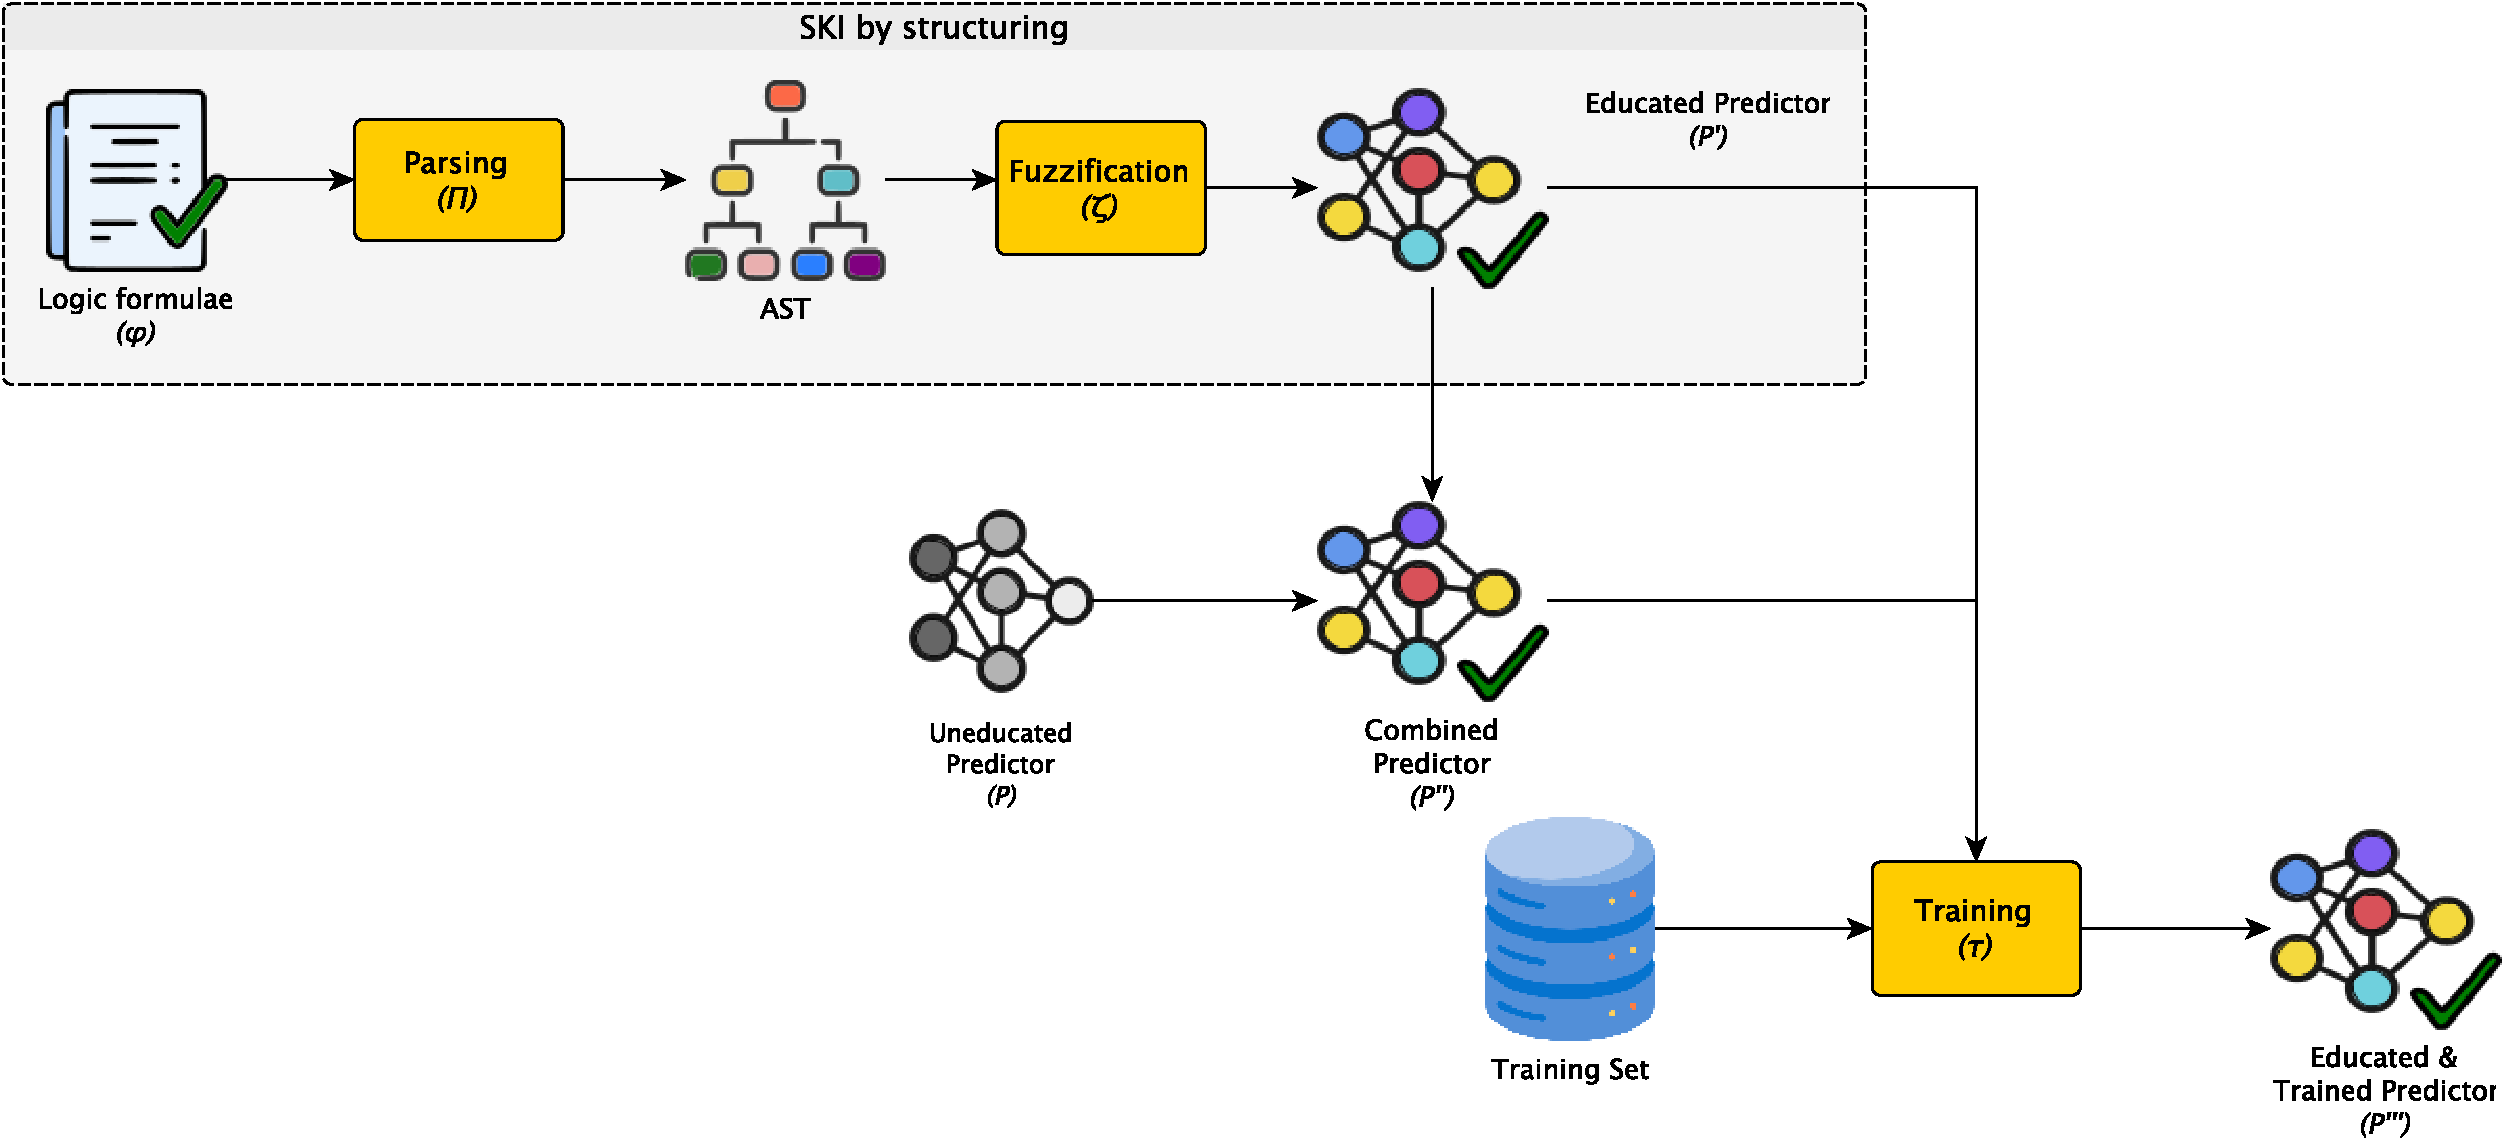
\includegraphics[width=.9\linewidth]{figures/workflow-structuring}
    \caption[SKI workflow of structuring strategy]{
        Workflow of the structuring strategy.
        %
        The symbolic knowledge is parsed and used to create a sub-symbolic predictor -- or part of it -- that mimics the symbolic knowledge.
        %
        The resulting predictor is then trained on data, if needed.
    }
    \label{fig:workflow-structuring}
\end{figure}
%
By predictor structuring, or simply structuring, we identify all those methods that use a part (or the whole) of a sub-symbolic predictor to \emph{mirror} the symbolic knowledge via its own internal structure.
%
A predictor is either created or extended to mimic the behavior of the symbolic knowledge.
%
For instance, when the predictors are \glspl{NN}, their internal structure is crafted to represent logic predicates via neurons, and logic connectives via synapses.
%
\Cref{fig:workflow-structuring} illustrates the workflow of the structuring strategy.
%
Usually, in the structuring strategy, the symbolic knowledge is in the form of logic formulas ($\phi$) (e.g., subsets of \gls{FOL}).
%
The formulas are then parsed into a syntactic structure (e.g., \gls{AST}).
%
At this point, a \emph{fuzzification} ($\zeta$) step is performed to convert the \emph{boolean} (also the term \emph{crisp} is used in the literature) -- because a logic predicate is either \emph{true} or \emph{false} -- symbolic knowledge into a \emph{fuzzy} interpretation of it, which is more suitable for sub-symbolic predictors.
%
This fuzzy interpretation is often \emph{continuous} and bounded to a predefined range, such as \([0, 1]\).
%
The property of continuity is a key requirement for training sub-symbolic structures via gradient descent (e.g., \glspl{NN} or part of them).
%
In practice, $\zeta$ is implemented as a mapping function that transforms logic operators into continuous functions (see \Cref{sec:from-symbolic-to-sub-symbolic}).
%
The result of the fuzzification process is an \emph{uneducated} predictor ($P$) that is then trained on the training set.
%
After the training, the predictor is now \emph{educated} ($P'$) and can be used to make predictions on the test set or in production.
%

\paragraph{Guided learning}\label{par:guided-learning}
%
\begin{figure}
    \centering
    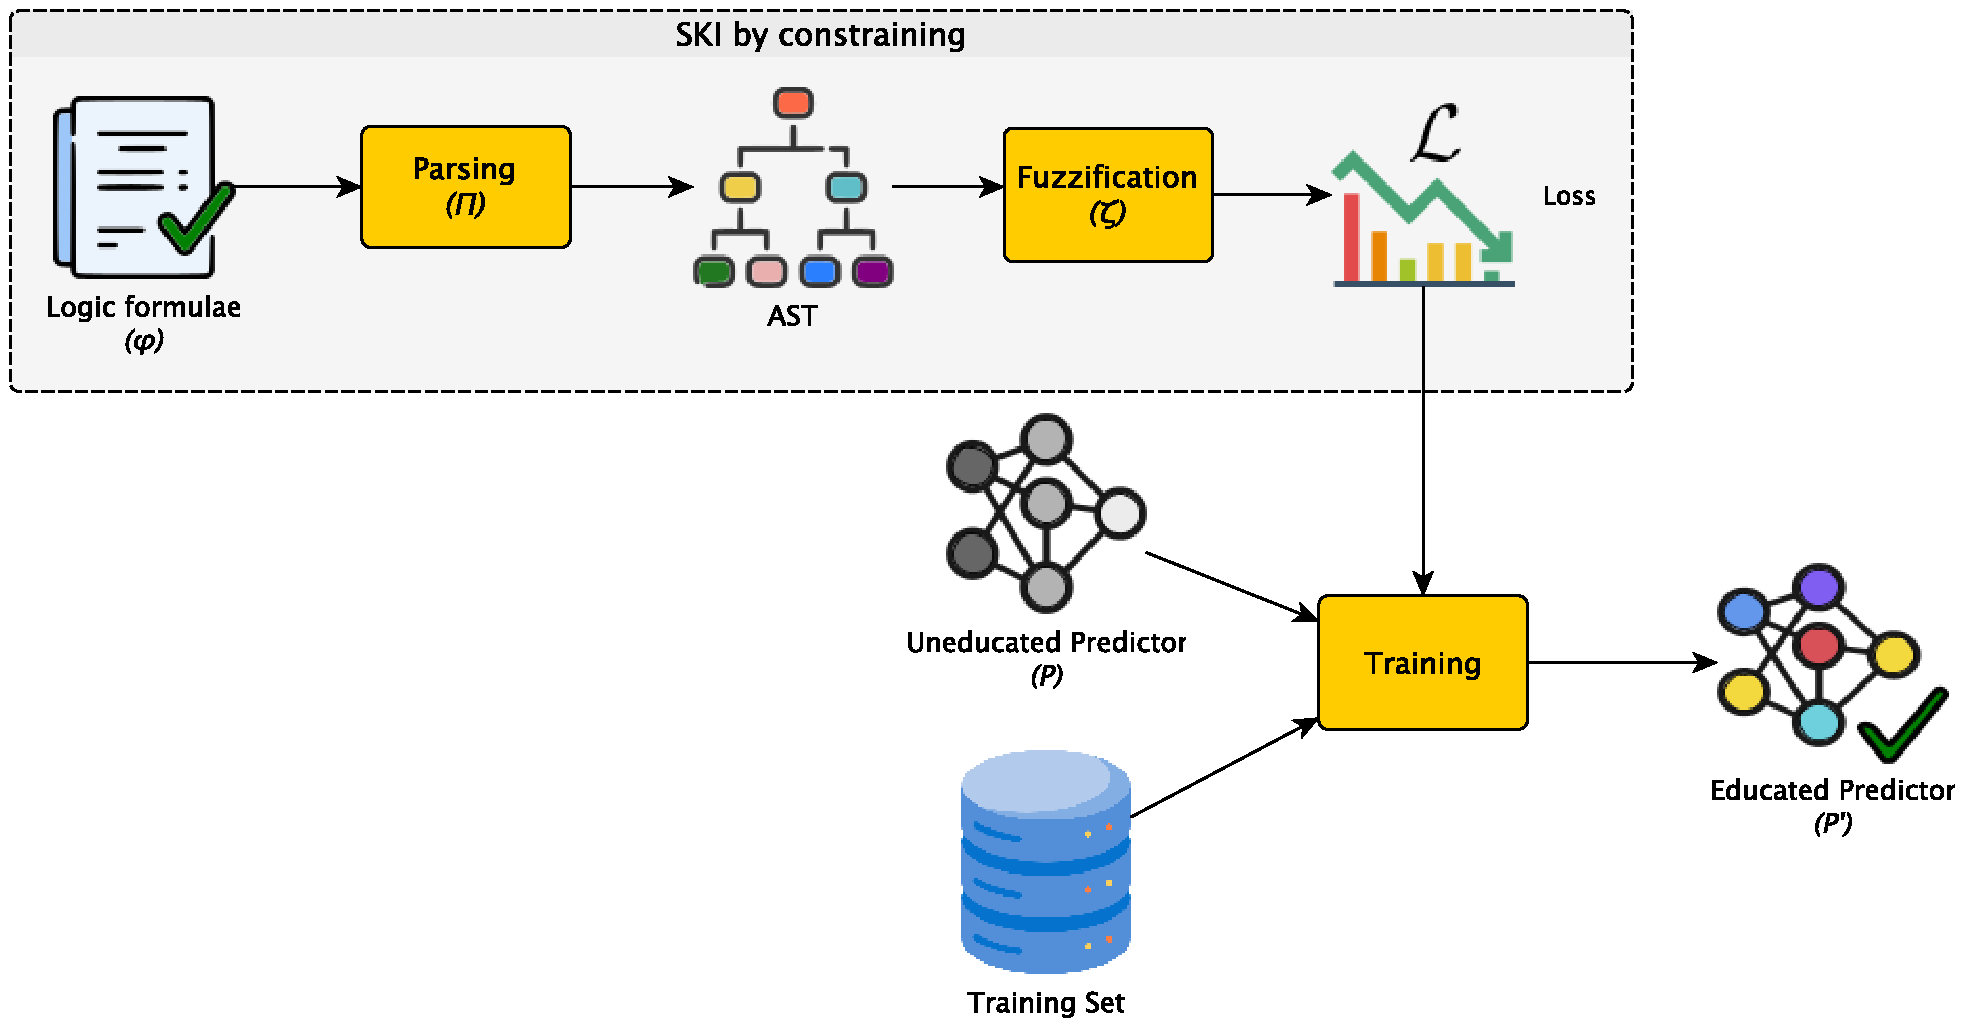
\includegraphics[width=.9\linewidth]{figures/workflow-constraining}
    \caption[SKI workflow of guided learning strategy]{
        \gls{SKI} workflow of the guided learning strategy.
        %
        The symbolic knowledge is used to guide the training of a sub-symbolic predictor, which is then trained on data.
    }
    \label{fig:workflow-learning}
\end{figure}
%
By guided learning, we refer to all those methods that affect the sub-symbolic predictor's training process by using the symbolic knowledge as a \emph{constraint}/\emph{guidance}.
%
Usually, \gls{SKI} algorithms based on this strategy target sub-symbolic predictors that can be trained with gradient descent, such as \glspl{NN}.
%
\Cref{fig:workflow-learning} illustrates the workflow of the guided learning strategy.
%
Like in the case of structuring, the symbolic knowledge is parsed and fuzzified.
%
Differently from structuring, the result of the fuzzification process is not a subcomponent of the predictor's architecture (e.g., neurons, connections), but rather a set of continuous numeric functions.
%
Conceptually, these functions represent the degree of violation of the symbolic knowledge by the predictor's predictions.
%
The higher the degree of violation, the higher the value of the function.
%
The symbolic-derived functions are then included in the loss function of the predictor, which is then trained on the training set.
%
The combination between the ``classical'' loss function (e.g., cross-entropy, mean squared error, etc.) and the symbolic-derived functions can be done in many ways, but it is usually done via a weighted sum.


\paragraph{Embedding}\label{par:ski-embedding}
%
\begin{figure}
    \centering
    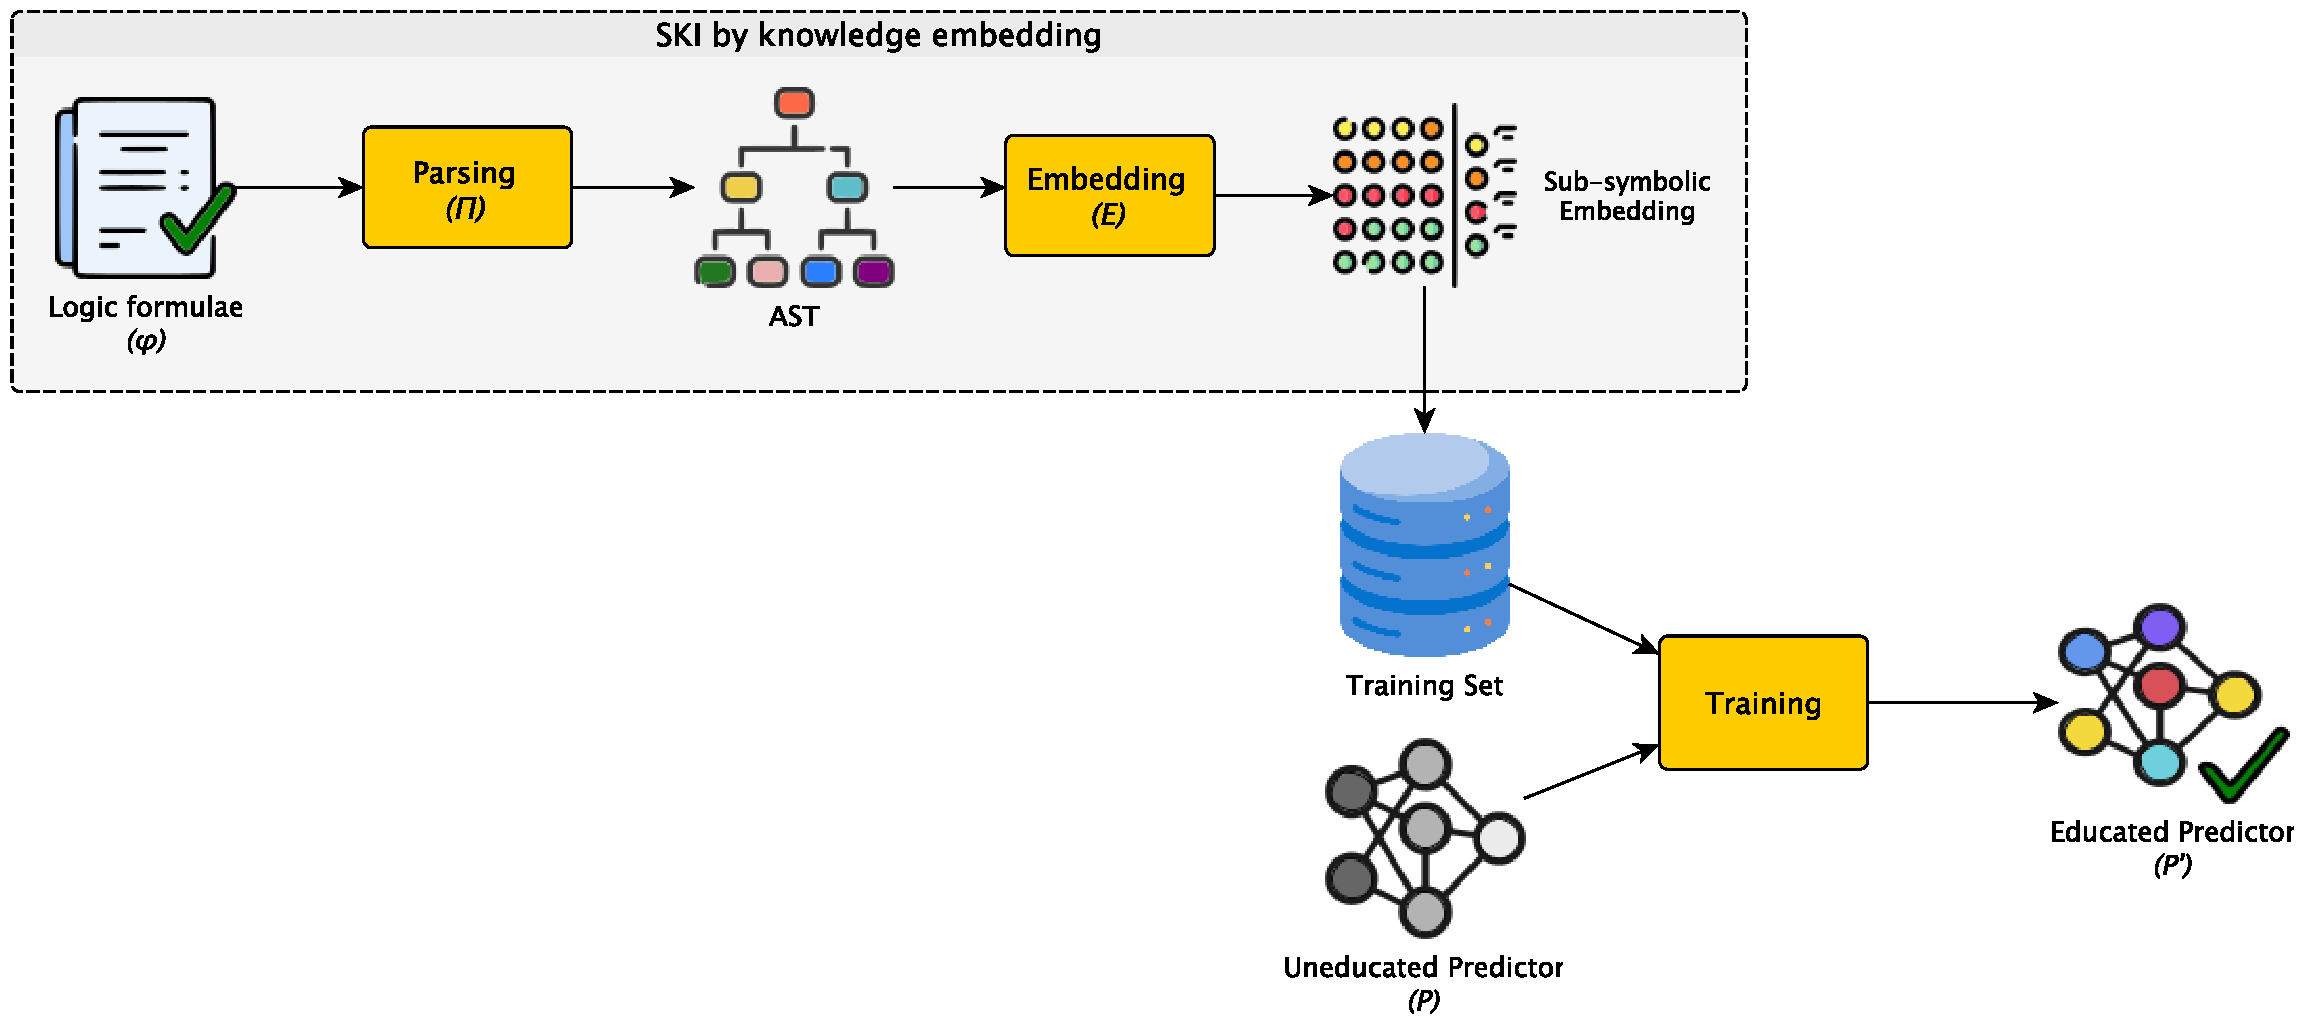
\includegraphics[width=.9\linewidth]{figures/workflow-embedding}
    \caption[SKI workflow of embedding strategy]{
        \gls{SKI} workflow of the embedding strategy.
        %
        The symbolic knowledge is parsed and embedded into a sub-symbolic predictor, which is then trained on data.
    }
    \label{fig:workflow-embedding}
\end{figure}
%
In the embedding strategy, the symbolic knowledge is converted -- i.e., \emph{embedded}-- into numeric-array representations.
%
\Cref{fig:workflow-embedding} illustrates the workflow of the embedding strategy.
%
The output of the fuzzification process is a set of numeric arrays (e.g., vectors, matrices, and tensors) that represent the symbolic knowledge.
%
These arrays are then provided as input to the sub-symbolic predictor.
%
This is the common strategy exploited by the \gls{KG}~\cite{DBLP:conf/ijcai/LambGGPAV20} embedding community as well as by \glspl{GNN}~\cite{DBLP:journals/tkde/WangMWG17}.


\subsection[Limitations and challenges of SKI]{Limitations and challenges of \Gls{SKI}}\label{subsec:limitations-and-challenges-of-ski}


\section[Symbolic knowledge extraction]{\Glsentrylong{SKE}}\label{sec:ske}
%
\gls{SKE} is the process of extracting symbolic knowledge from sub-symbolic predictors.
%
Here, we provide the broad definition of \gls{SKE} that we adopt in this thesis:
%
\begin{definition}[\gls{SKE}]
    \label{def:ske}
    any \textbf{algorithmic} procedure accepting \textbf{trained} sub-symbolic predictors as input and producing \textbf{symbolic} knowledge as output so that the extracted knowledge reflects the behavior of the predictor with high \textbf{fidelity}~\cite{DBLP:journals/csur/CiattoSAMO24}.
\end{definition}
%
Once again, the definition is broad because the amount of contributions in the literature is vast and varied, they often use different terminologies and come from different communities.
%
\Gls{SKE} is conceptualized as a class of algorithms, which are finite-step procedures defined by their inputs and outputs.

The input to \gls{SKE} procedures must be trained \glspl{ML} predictors.
%
There are no restrictions on the type of predictor, meaning that \gls{SKE} methods can, in principle, be applied to any predictor family.
%
However, this requirement implies that the predictor must have already undergone training and achieved satisfactory performance for its intended task.
%
Thus, within an \gls{ML} workflow, \gls{SKE} is performed after the training and validation phases are complete.

The output of \gls{SKE} procedures is symbolic knowledge, which is broadly defined as human-intelligible information.
%
This can include logic formulas, decision trees, or even plain human-readable text.
%
For an algorithm to qualify as a valid \gls{SKE} procedure, the extracted knowledge must closely reflect the behavior of the original predictor within the domain it was trained for.
%
This fidelity is typically measured using a fidelity score, which evaluates how well the extracted knowledge replicates the predictor's behavior for the given task and domain.

The extracted knowledge should ideally function as a predictor itself, allowing it to be queried in the same way as the original predictor.
%
For example, if the original predictor is an image classifier, the extracted knowledge should enable an intelligent agent to classify similar images and produce equivalent results.
%
This agent could be either computational (e.g., a software program) or human, depending on whether the extracted knowledge is machine- or human-interpretable.
%
The use of logic-based knowledge as the target of \gls{SKE} is particularly advantageous, as it supports both machine and human interpretability.


\subsection{Motivations and goals}\label{subsec:ske-motivations-and-goals}

\subsection{How to extract}\label{subsec:how-to-extract}

\subsection[Decompositional SKE]{Decompositional \Gls{SKE}}\label{subsec:decompositional-ske}

\subsection[Pedagocial SKE]{Pedagocial \Gls{SKE}}\label{subsec:pedagogical-ske}

\subsection{Local explanations}\label{subsec:local-explanations}

\subsection{Global explanations}\label{subsec:global-explanations}

\subsection[Limitations and challenges of SKE]{Limitations and challenges of \Gls{SKE}}\label{subsec:limitations-and-challenges-of-ske}
%! Author = matteomagnini
%! Date = 05/03/25

%----------------------------------------------------------------------------------------
\chapter{Large Language Models}
\label{ch:llm}
\mtcaddchapter
\minitoc
%----------------------------------------------------------------------------------------

\section{Architectures}\label{sec:llm-architectures}

\subsection{Transformer}\label{subsec:transformer}

\subsection{Attention}\label{subsec:attention}

\section{Fine-tuning}\label{sec:llm-fine-tuning}

\section{\Glsentrylong{RAG}}\label{sec:rag}

\subsection{Embedding}\label{subsec:rag-embedding}

\subsection{Retrieval}\label{subsec:retrieval}

\section{Limitations and challenges}\label{sec:limitations-and-challenges}

\subsection{Resources}\label{subsec:resources}

\subsection{Data and privacy}\label{subsec:data-and-privacy}

\subsection{Hallucinations}\label{subsec:hallucinations}

\subsection{Stochastic parrot or something more?}\label{subsec:stochastic-parrot-or-something-more}

%----------------------------------------------------------------------------------------
%--------------------------------------- PART II-----------------------------------------
%----------------------------------------------------------------------------------------

\part{Engineering of \ac{SKI} \& \ac{SKE}}\label{part:engineering-of-ski-ske}

\chapter{Common patterns}\label{ch:common-patterns}

\section{Knowledge representation}\label{sec:knowledge-representation}

\subsection{Logic rules}\label{subsec:logic-rules}

\subsection{\Aclp{KG}}\label{subsec:kg}

\subsection{Free text}\label{subsec:free-text}

\section{From symbolic to sub-symbolic}\label{sec:from-symbolic-to-sub-symbolic}

\subsection{Fuzzyfication}\label{subsec:fuzzyfication}

\subsection{Delegation}\label{subsec:delegation}

\section{From sub-symbolic to symbolic}\label{sec:from-sub-symbolic-to-symbolic}

\subsection{Surrogate models}\label{subsec:surrogate-models}

\subsection{De-fuzzyfication}\label{subsec:unfuzzyfication}

%----------------------------------------------------------------------------------------

\chapter{\Acl{PSyKI}}\label{ch:psyki}

\section{Implementation}\label{sec:implementation}

\subsection{Goals}\label{subsec:goals}

\subsection{Architecture}\label{subsec:architecture}

\subsection{Details}\label{subsec:details}

\section{Available \ac{SKI} methods}\label{sec:available-ski-methods}

\subsection{\Acl{KBANN}}\label{subsec:kbann}

\subsection{\Acl{KINS}}\label{subsec:kins}

\subsection{\Acl{KILL}}\label{subsec:kill}

\section{\Acl{QoS} for \ac{SKI}}\label{sec:qos}

\section{Fairness}\label{sec:fairness}

\subsection{\Acl{FaUCI}}\label{subsec:fauci}

%----------------------------------------------------------------------------------------
%----------------------------------------------------------------------------------------

\part{Engineering of intelligent systems}\label{part:engineering-of-intelligent-systems}

%----------------------------------------------------------------------------------------
%----------------------------------------------------------------------------------------

\chapter{\Ac{NeSy} \ac{AI} for real world applications}\label{ch:nesy-ai-for-real-world-applications}

\section{Motivations}\label{sec:nesy-ai-motivations}

\section{Goals and challenges}\label{sec:nesy-ai-goals-and-challenges}

\section{Applications}\label{sec:nesy-ai-applications}

\subsection{\Ac{SKE} for explainable nutritional recommenders}\label{subsec:ske-for-explainable-nutritional-recommenders}

\subsection{A general-purpose protocol for multi-agent based explanations}\label{subsec:a-general-purpose-protocol-for-multi-agent-based-explanations}

\subsection{\Acl{NeSy} \ac{AI} for supporting chronic disease diagnosis and monitoring}\label{subsec:nesy-ai-for-supporting-chronic-disease-diagnosis-and-monitoring}

\subsection{\Ac{LLM}-based solutions for healthcare chatbots: a comparative analysis}\label{subsec:llm-based-solutions-for-healthcare-chatbots-a-comparative-analysis}

\subsection{Open-source small language models for personal medical assistant chatbots}\label{subsec:open-source-small-language-models-for-personal-medical-assistant-chatbots}

\subsection{Applying \acl{RAG} on open \acp{LLM} for a medical chatbot supporting hypertensive patients}\label{subsec:applying-rag-on-open-llm-for-a-medical-chatbot-supporting-hypertensive-patients}

%----------------------------------------------------------------------------------------

\chapter{Autonomous learning systems}\label{ch:autonomous-learning-systems}

\section{Motivations}\label{sec:motivations}

\section{Goals and challenges}\label{sec:goals-and-challenges}

\section{Applications}\label{sec:applications}

\subsection{Actively learning ontologies from \acp{LLM}}\label{subsec:exact-learning-with-ac{llm}}

\subsection{\Aclp{LLM} as oracles for instantiating ontologies with domain-specific knowledge}\label{subsec:llm-as-oracles-for-instantiating-ontologies-with-domain-specific-knowledge}

%----------------------------------------------------------------------------------------

\chapter{Conclusions}\label{ch:conclusions}

\section{Discussion}\label{sec:discussion}

\section{Future work}\label{sec:future-work}

%----------------------------------------------------------------------------------------
% BIBLIOGRAPHY
%----------------------------------------------------------------------------------------

\backmatter

\part*{}

\nocite{*} % comment this to only show the referenced entries from the .bib file
\bibliographystyle{alpha}
\bibliography{phd-thesis}

\end{document}